\subsection{Etap Build}
Faza budowania (\textit{Build}) odpowiada za przekształcenie kodu źródłowego w~gotowe do wdrożenia artefakty. W~architekturze \textit{Cloud Native} proces ten kończy się wytworzeniem obrazu kontenera.

\subsubsection{Orkiestracja procesu CI/CD: GitHub Actions}
Zgodnie z~decyzją \textit{ADR-0009}, jako platformę CI/CD wybrano \textbf{GitHub Actions}. Pozwala ona na definiowanie procesów CI/CD w~formie kodu YAML bezpośrednio w~repozytorium, co jest zgodne z~zasadą \textit{Everything as Code} i~eliminuje potrzebę utrzymywania zewnętrznego serwera CI.

\textbf{Rola w~projekcie:}
GitHub Actions pełni funkcję silnika CI (\textit{Continuous Integration}), który reaguje na zdarzenia w~repozytorium (np. \textit{pull request} lub \textit{push} do gałęzi głównej). Proces CI/CD automatycznie uruchamia kompilację, testy oraz budowanie obrazów, zapewniając szybką pętlę informacji zwrotnej dla programisty.

\textbf{Struktura procesów CI/CD:}
Dla każdego mikroserwisu zdefiniowano oddzielny plik \textit{workflow} (np. \texttt{ci-users.yml}), uruchamiany wyłącznie przy zmianach w~katalogu danego serwisu. Takie podejście eliminuje zbędne uruchomienia procesu CI dla komponentów, których kod nie uległ zmianie.

\begin{lstlisting}[language=yaml, caption={Fragment procesu CI --- budowanie i~push obrazu natywnego (.github/workflows/ci-users.yml)}, label={lst:github-actions-build}]
jobs:
  build:
    name: Build, Test, Scan & Push — users
    runs-on: ubuntu-latest
    permissions:
      contents: read
      id-token: write   # wymagane przez Cosign keyless signing
    steps:
      - uses: actions/checkout@v7
      - name: Set up JDK 25
        uses: actions/setup-java@v5
        with:
          java-version: '25'
          distribution: temurin
          cache: gradle
      - name: Run tests
        run: ./gradlew :apps:users:test --no-daemon
      - name: Build application and container image
        run: |
          ./gradlew :apps:users:imageBuild \
            -Dquarkus.container-image.tag=${{ github.sha }} \
            --no-daemon
\end{lstlisting}

Pełny przebieg procesu CI --- od zdarzenia w~repozytorium, przez testy i~budowanie obrazu natywnego, po bramkę skanowania i~podpis artefaktu --- przedstawia rysunek~\ref{fig:ci-pipeline}. Rysunek~\ref{fig:ci-governance} pokazuje ten sam proces z~perspektywy zdarzeń: bieg dla \textit{pull requesta} jedynie waliduje zmiany, a~dopiero bieg dla gałęzi \texttt{main} publikuje i~podpisuje obraz; ochrona gałęzi blokuje scalenie do czasu pomyślnego zakończenia weryfikacji CI.

\begin{figure}[H]
    \centering
    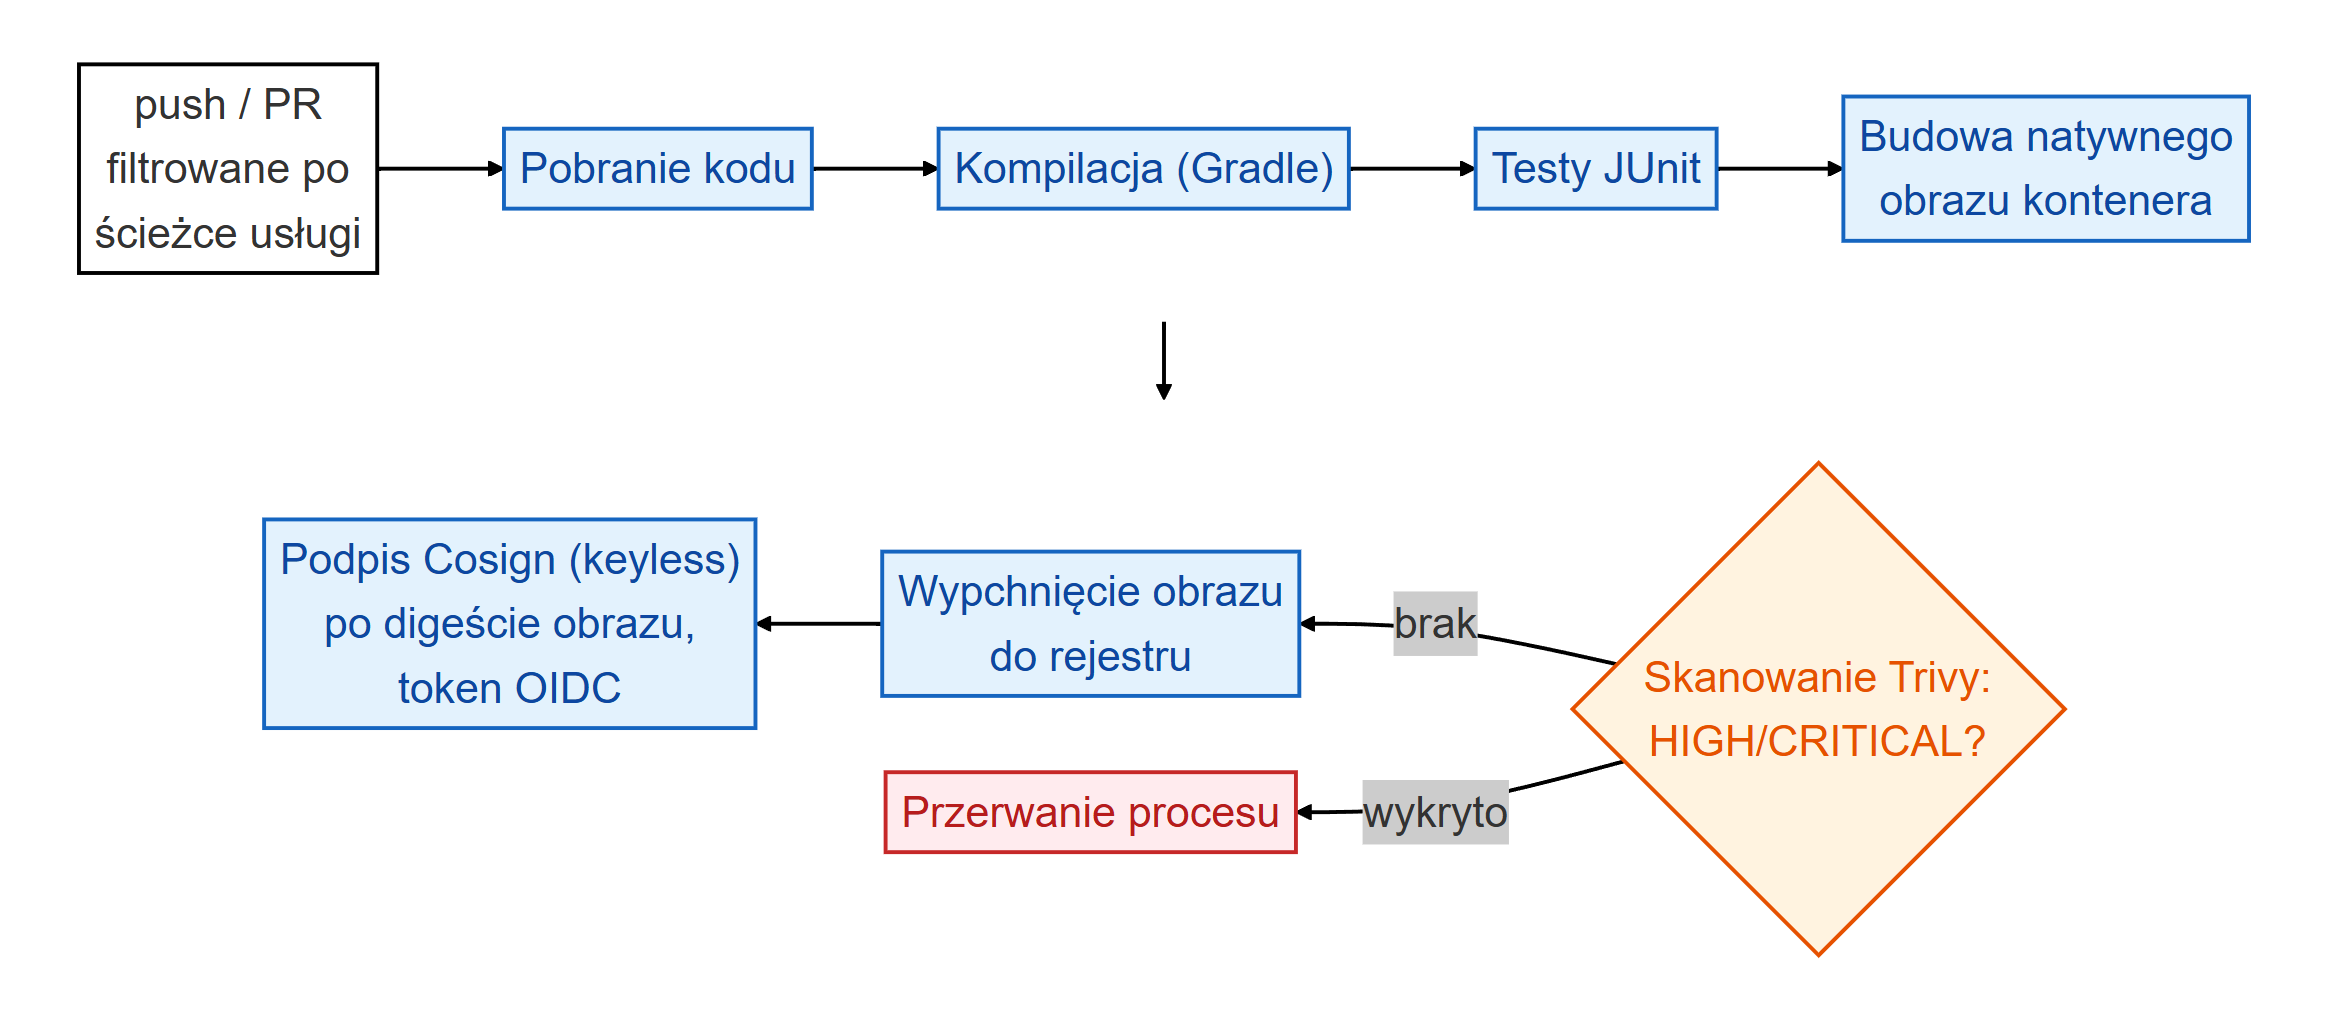
\includegraphics[width=\textwidth]{img/diagrams/04-build/build-01-ci-pipeline.png}
    \caption{Proces CI z~bezpieczeństwem Shift-Left --- skanowanie Trivy jako bramka przed publikacją, podpis Cosign po wypchnięciu obrazu (por.\ rys.~\ref{fig:ci-governance}; opracowanie własne).}
    \label{fig:ci-pipeline}
\end{figure}

\begin{figure}[H]
    \centering
    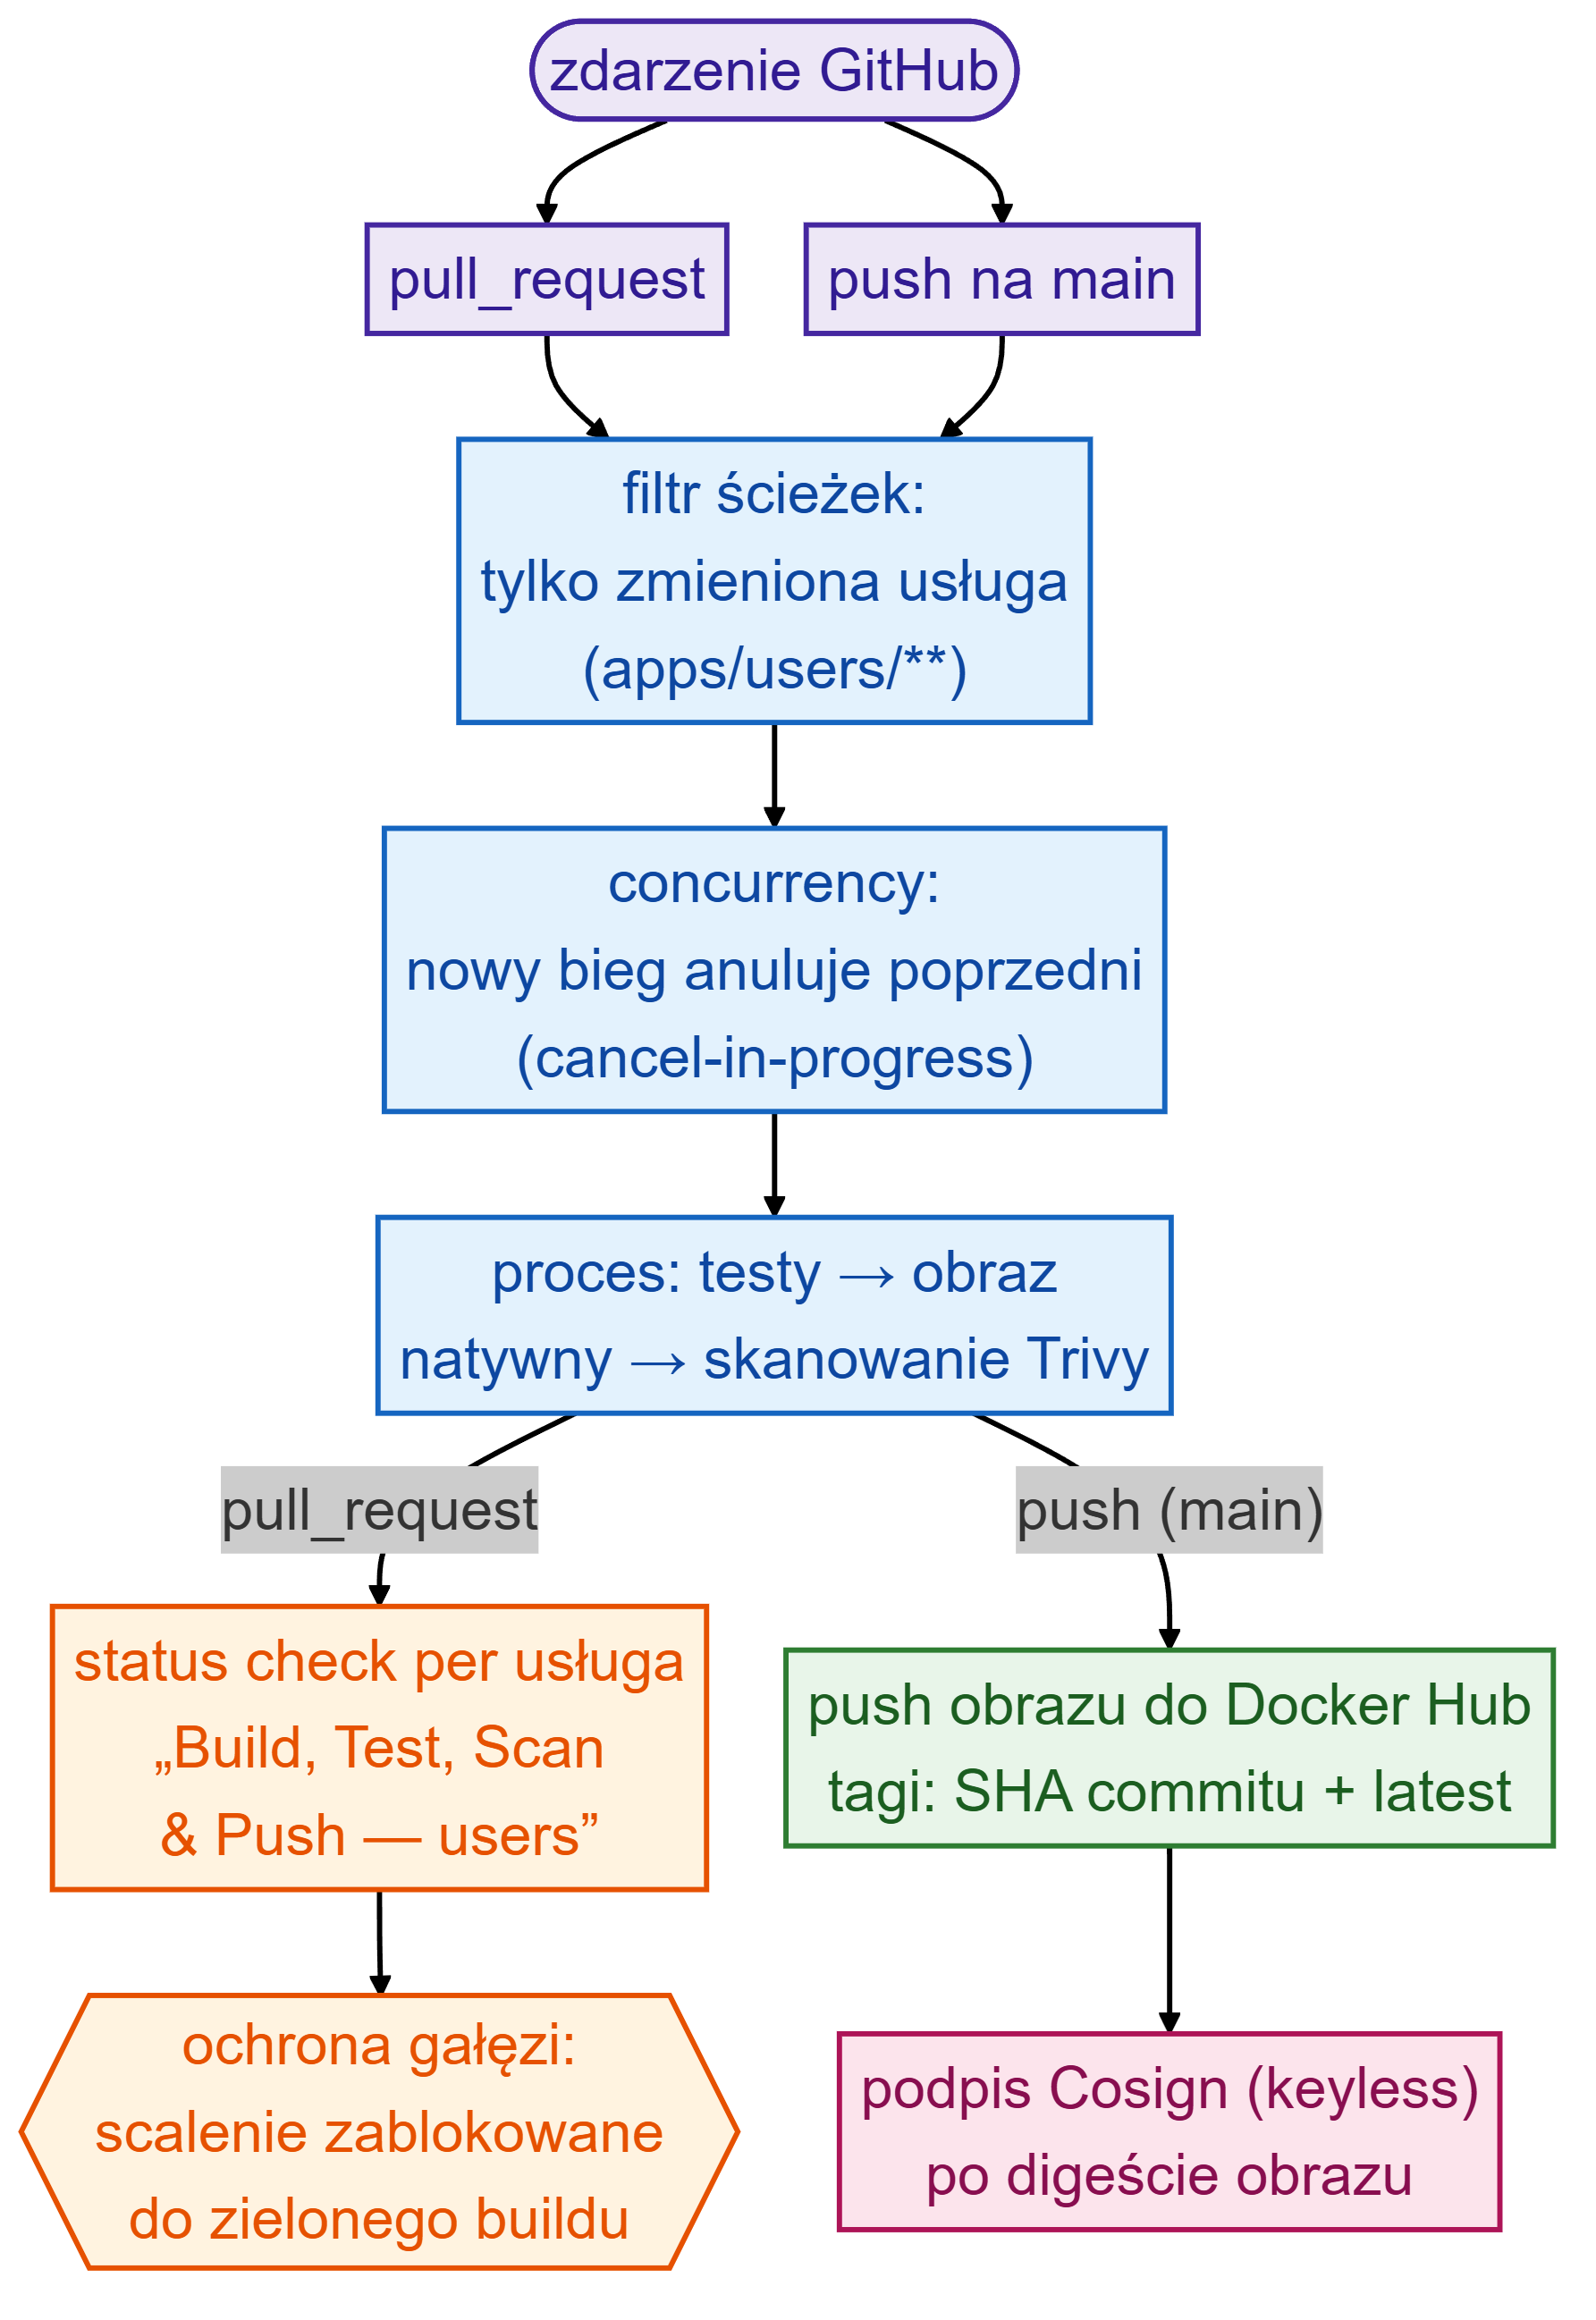
\includegraphics[width=0.6\textwidth]{img/diagrams/04-build/build-02-flow-ci-governance.png}
    \caption{Zdarzenia i~bramki tego samego procesu --- walidacyjny bieg \textit{pull requesta} i~publikujący bieg \texttt{main} z~ochroną gałęzi (por.\ rys.~\ref{fig:ci-pipeline}; opracowanie własne).}
    \label{fig:ci-governance}
\end{figure}

\subsubsection{Budowanie artefaktów: Gradle i~NPM}
W~zależności od komponentu wykorzystywane są wyspecjalizowane narzędzia budujące:
\begin{itemize}
    \item \textbf{Gradle (Backend):} Zarządza zależnościami projektu Java/Quarkus, kompiluje kod oraz uruchamia testy jednostkowe. Wybrano go (ADR-0008) ze względu na elastyczność i~wydajność (mechanizm \textit{build cache}).
    \item \textbf{Vite (Frontend):} Odpowiada za budowanie zoptymalizowanej paczki produkcyjnej aplikacji Vue 3. Vite wykorzystuje natywne moduły ES podczas prac programistycznych, co skraca czas przeładowania do milisekund, a~NPM zarządza zależnościami projektu.
\end{itemize}

\subsubsection{Konteneryzacja: Docker + Dockerfile}
Zgodnie z~decyzją \textit{ADR-0005}, jako standard budowania obrazów wybrano pliki \textbf{Dockerfile}. Wybór ten podyktowany był chęcią zachowania pełnej przejrzystości procesu, co ma kluczowe znaczenie w~pracy inżynierskiej.

\begin{techcard}{Docker}

\textbf{Opis:} Docker to platforma konteneryzacji pozwalająca na pakowanie oprogramowania wraz z~całym środowiskiem uruchomieniowym w~lekkie, przenośne kontenery. Dzięki temu aplikacja działa identycznie niezależnie od maszyny docelowej.

\textbf{Dobre nawyki:}
\begin{itemize}
  \item \textbf{Multi-stage builds:} Oddzielenie środowiska kompilacji od uruchomieniowego redukuje rozmiar końcowego obrazu i~eliminuje narzędzia budujące z~obrazu produkcyjnego.
  \item \textbf{Zasada najniższych uprawnień:} Kontenery nie powinny działać jako użytkownik \texttt{root} --- należy zdefiniować wydzielonego użytkownika technicznego (patrz listing \ref{lst:dockerfile-native}).
  \item \textbf{Precyzyjne tagowanie:} Unikanie tagu \texttt{latest} na rzecz konkretnych wersji (semantycznych lub hashów git) zapewnia powtarzalność wdrożeń.
  \item \textbf{Plik \texttt{.dockerignore}:} Wykluczanie zbędnych plików (np. \texttt{node\_modules}, \texttt{.git}, \texttt{target/}) przyspiesza budowanie i~zapobiega wyciekom danych wrażliwych.
\end{itemize}

\textbf{Rola w~projekcie:} Docker pełni rolę „pakowacza” --- przed jego użyciem dostępny jest skompilowany plik binarny, a~po zbudowaniu obrazu powstaje gotowy do wdrożenia artefakt uruchamialny w~dowolnym środowisku kontenerowym. Dockerfile dla trybu natywnego przedstawia listing \ref{lst:dockerfile-native}.

\end{techcard}

\textbf{Docker i~Quarkus --- kompilacja AOT i~minimalne obrazy:}
Quarkus generuje gotowe pliki \texttt{Dockerfile.native} przeznaczone dla obrazów zbudowanych w~trybie GraalVM \textit{Ahead-of-Time} (AOT). Kompilacja natywna odbywa się wewnątrz kontenera Mandrel (dystrybucja GraalVM zoptymalizowana pod kątem Quarkusa) uruchamianego przez Gradle w~procesie CI, bez konieczności instalowania GraalVM bezpośrednio na maszynie CI. Konfigurację narzędzia budującego zawiera plik \texttt{build.gradle}:

\begin{lstlisting}[language=groovy, caption={Konfiguracja natywnego buildu Quarkusa w~Gradle (apps/users/build.gradle)}, label={lst:quarkus-native-build}]
quarkusBuild {
    nativeArgs {
        containerBuild = true
        builderImage = "quay.io/quarkus/ubi10-quarkus-mandrel-builder-image:jdk-25"
    }
}
\end{lstlisting}

Wynikiem kompilacji jest samodzielny plik wykonywalny (\texttt{build/*-runner}), który nie wymaga środowiska JVM. Dockerfile kopiuje go do minimalnego obrazu bazowego Red Hat UBI:

\begin{lstlisting}[language=docker, caption={Natywny Dockerfile Quarkusa dla mikroserwisu \textit{users} (apps/users/src/main/docker/Dockerfile.native)}, label={lst:dockerfile-native}]
FROM registry.access.redhat.com/ubi10/ubi-minimal:10.2
WORKDIR /work/
RUN chown 1001 /work \
    && chmod "g+rwX" /work \
    && chown 1001:root /work
COPY --chown=1001:root --chmod=0755 build/*-runner /work/application

EXPOSE 8080
USER 1001

ENTRYPOINT ["./application", "-Dquarkus.http.host=0.0.0.0"]
\end{lstlisting}

Obraz końcowy zawiera wyłącznie minimalny system operacyjny i~skompilowany plik binarny aplikacji --- bez JVM, JDK ani żadnych narzędzi budujących. Warstwa frontendowa (\textit{Vue 3}) stosuje klasyczny wzorzec wieloetapowy: etap kompilacji Vite produkujący statyczne pliki w~katalogu \texttt{dist/}, a~następnie serwowanie ich przez minimalny obraz \textit{nginx}.
Całą ścieżkę budowania natywnego --- na tle klasycznej ścieżki JVM --- podsumowuje rysunek~\ref{fig:native-build}: kosztem długiej kompilacji AOT (analiza zamkniętego świata --- założenie, że cały kod potrzebny w~czasie działania jest znany w~chwili kompilacji) uzyskuje się start w~milisekundach oraz minimalny obraz pozbawiony środowiska JVM.

\begin{figure}[H]
    \centering
    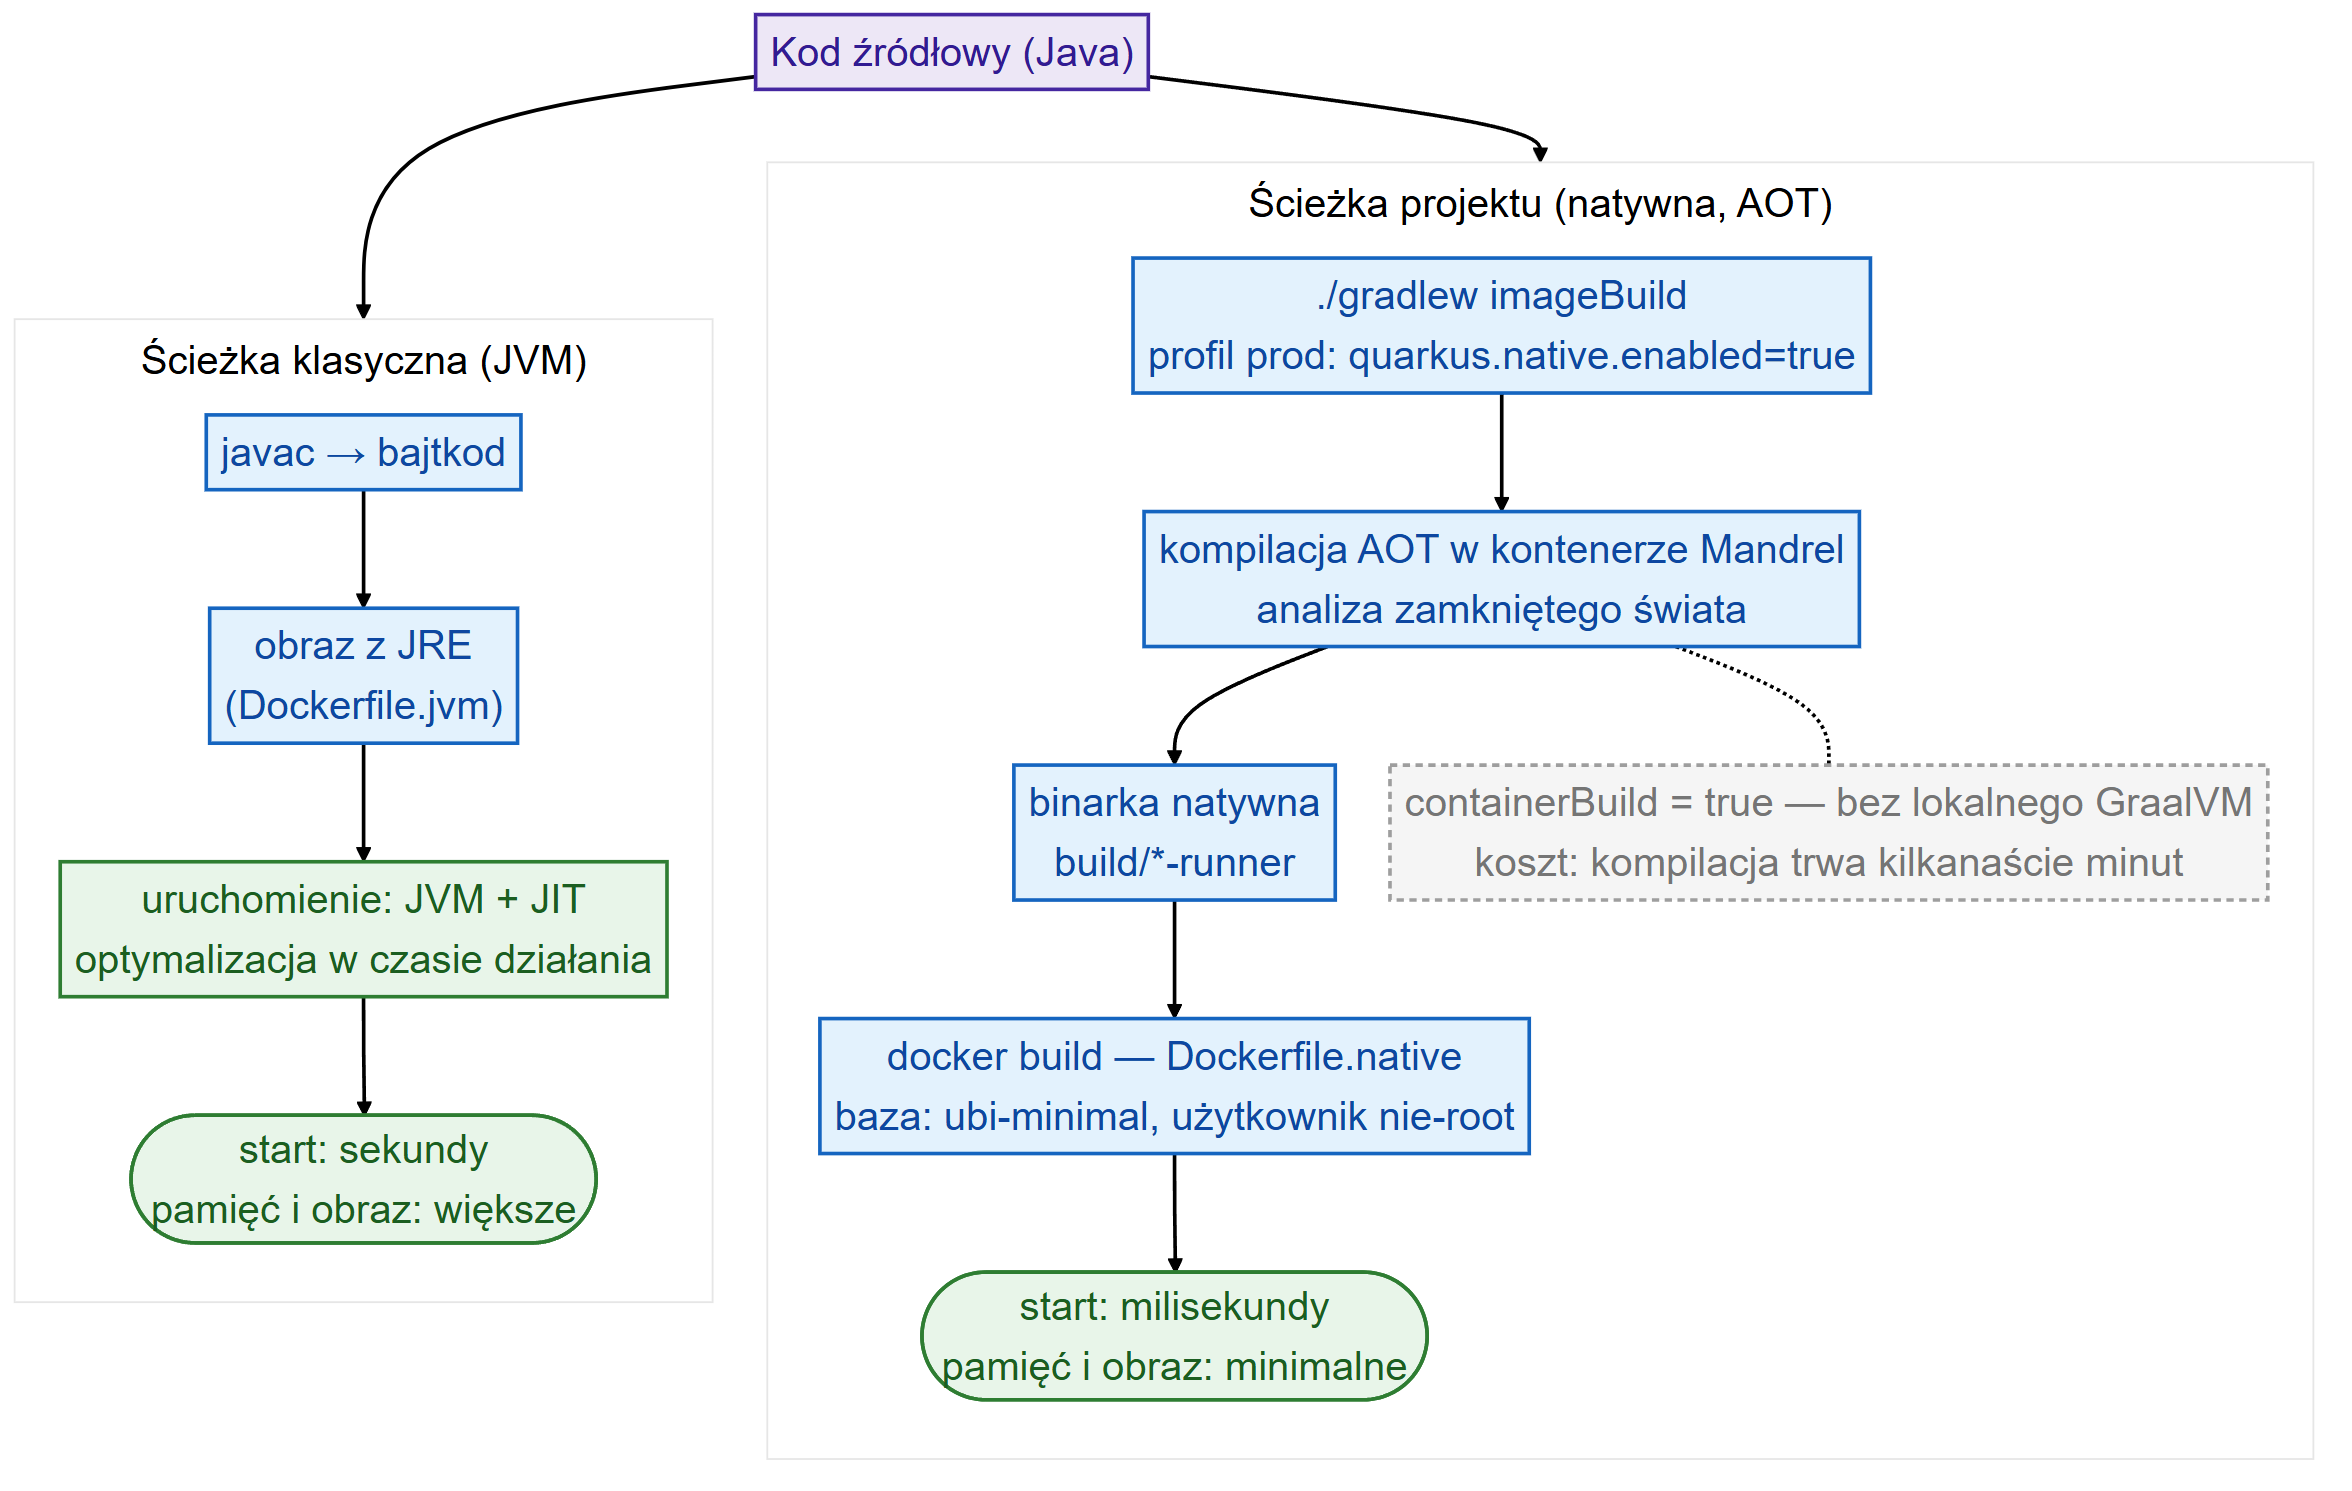
\includegraphics[width=\textwidth]{img/diagrams/04-build/build-03-flow-native-build.png}
    \caption{Anatomia budowania natywnego --- ścieżka klasyczna (JVM, optymalizacja JIT w~czasie działania) na tle ścieżki projektu (kompilacja AOT w~kontenerze Mandrel, minimalny obraz); koszt kompilacji wymieniony na szybki start i~małe zużycie pamięci (opracowanie własne).}
    \label{fig:native-build}
\end{figure}

\textbf{Shift-Left Security:}
Bezpieczeństwo jest weryfikowane już na etapie budowania:
\begin{itemize}
    \item \textbf{Trivy (ADR-0010):} Każdy zbudowany obraz jest skanowany pod kątem znanych podatności (CVE) w~bibliotekach systemowych i~aplikacyjnych.
\begin{lstlisting}[language=yaml, caption={Skanowanie obrazu narzędziem Trivy w~procesie CI (.github/workflows/ci-users.yml)}, label={lst:trivy-scan}]
- name: Scan image with Trivy
  uses: aquasecurity/trivy-action@v0.36.0
  with:
    image-ref: mateuszwas/users:${{ github.sha }}
    format: table
    exit-code: '1'
    ignore-unfixed: true
    vuln-type: os,library
    severity: HIGH,CRITICAL
\end{lstlisting}
    \item \textbf{Cosign (ADR-0011):} Obrazy są cyfrowo podpisywane metodą \textit{keyless signing} (Sigstore), co zapewnia ich integralność i~pozwala na weryfikację pochodzenia artefaktu przed jego uruchomieniem w~klastrze.
\end{itemize}
